
\renewcommand{\theequation}{\theenumi}
\begin{enumerate}[label=\arabic*.,ref=\thesubsection.\theenumi]
\numberwithin{equation}{enumi}
%
\item
	The area of the rectangle $ACBD$ shown in Fig. \ref{fig:tri_rect} is defined as $ac$. Note that all the angles in the rectangle are $90\degree$
%	\label{fig:tri_rect}

\begin{figure}[!ht]
	\begin{center}
		
		%\includegraphics[width=\columnwidth]{./figs/fig:tri_rect}
		%\vspace*{-10cm}
		\resizebox{\columnwidth}{!}{%Code by GVV Sharma
%December 7, 2019
%released under GNU GPL
%Drawing a rectangle

\begin{tikzpicture}
[scale=2,>=stealth,point/.style={draw,circle,fill = black,inner sep=0.5pt},]

%Triangle sides
\def\a{4}
\def\c{3}

%Marking coordiantes
\coordinate [label=above:$A$] (A) at (0,\c);
\coordinate [label=left:$B$] (B) at (0,0);
\coordinate [label=right:$C$] (C) at (\a,0);

%Drawing triangle ABC
\draw (A) -- node[left] {$\textrm{c}$} (B) -- node[below] {$\textrm{a}$} (C) -- node[above,,xshift=2mm] {$\textrm{b}$} (A);

\node (D) at (\a, \c)[point,label=above right:$D$] {};

%Joining AD and CD
\draw (A)--(D);
\draw (C)--(D);

%Drawing and marking angles
\tkzMarkRightAngle[fill=blue!20,size=.3](A,B,C)
\tkzMarkRightAngle[fill=blue!20,size=.3](A,D,C)
\end{tikzpicture}
}
	\end{center}
	\caption{Area of a Right Triangle}
	\label{fig:tri_rect}	
\end{figure}
%
\item Draw Fig. \ref{fig:tri_rect} for $a = 4, c =3$.
\label{const:tri_rect}
\\
\solution Letting
%
\begin{align}
\vec{B} = \myvec{0 \\  0}, 
\vec{D} = \myvec{4 \\  3} 
\label{eq:tri_rect}
\end{align}
%
the python code for  Fig. \ref{fig:tri_rect} is
\begin{lstlisting}
codes/triangle/tri_rect.py
\end{lstlisting}
%
and the equivalent latex-tikz code is
%
\begin{lstlisting}
figs/triangle/tri_rect.tex
\end{lstlisting}

\item
	The area of the two triangles constituting the rectangle is the same.
	\label{ch2_triang_eq}

\item
	The area of the rectangle is the sum of the areas of the two triangles inside.
	\label{ch2_triang_sum}


\item
\label{prob:ch2_triang_area}
	Show that the area of $\Delta ABC$ is $\frac{ac}{2}$

\begin{figure}[!ht]
	\begin{center}
		
		%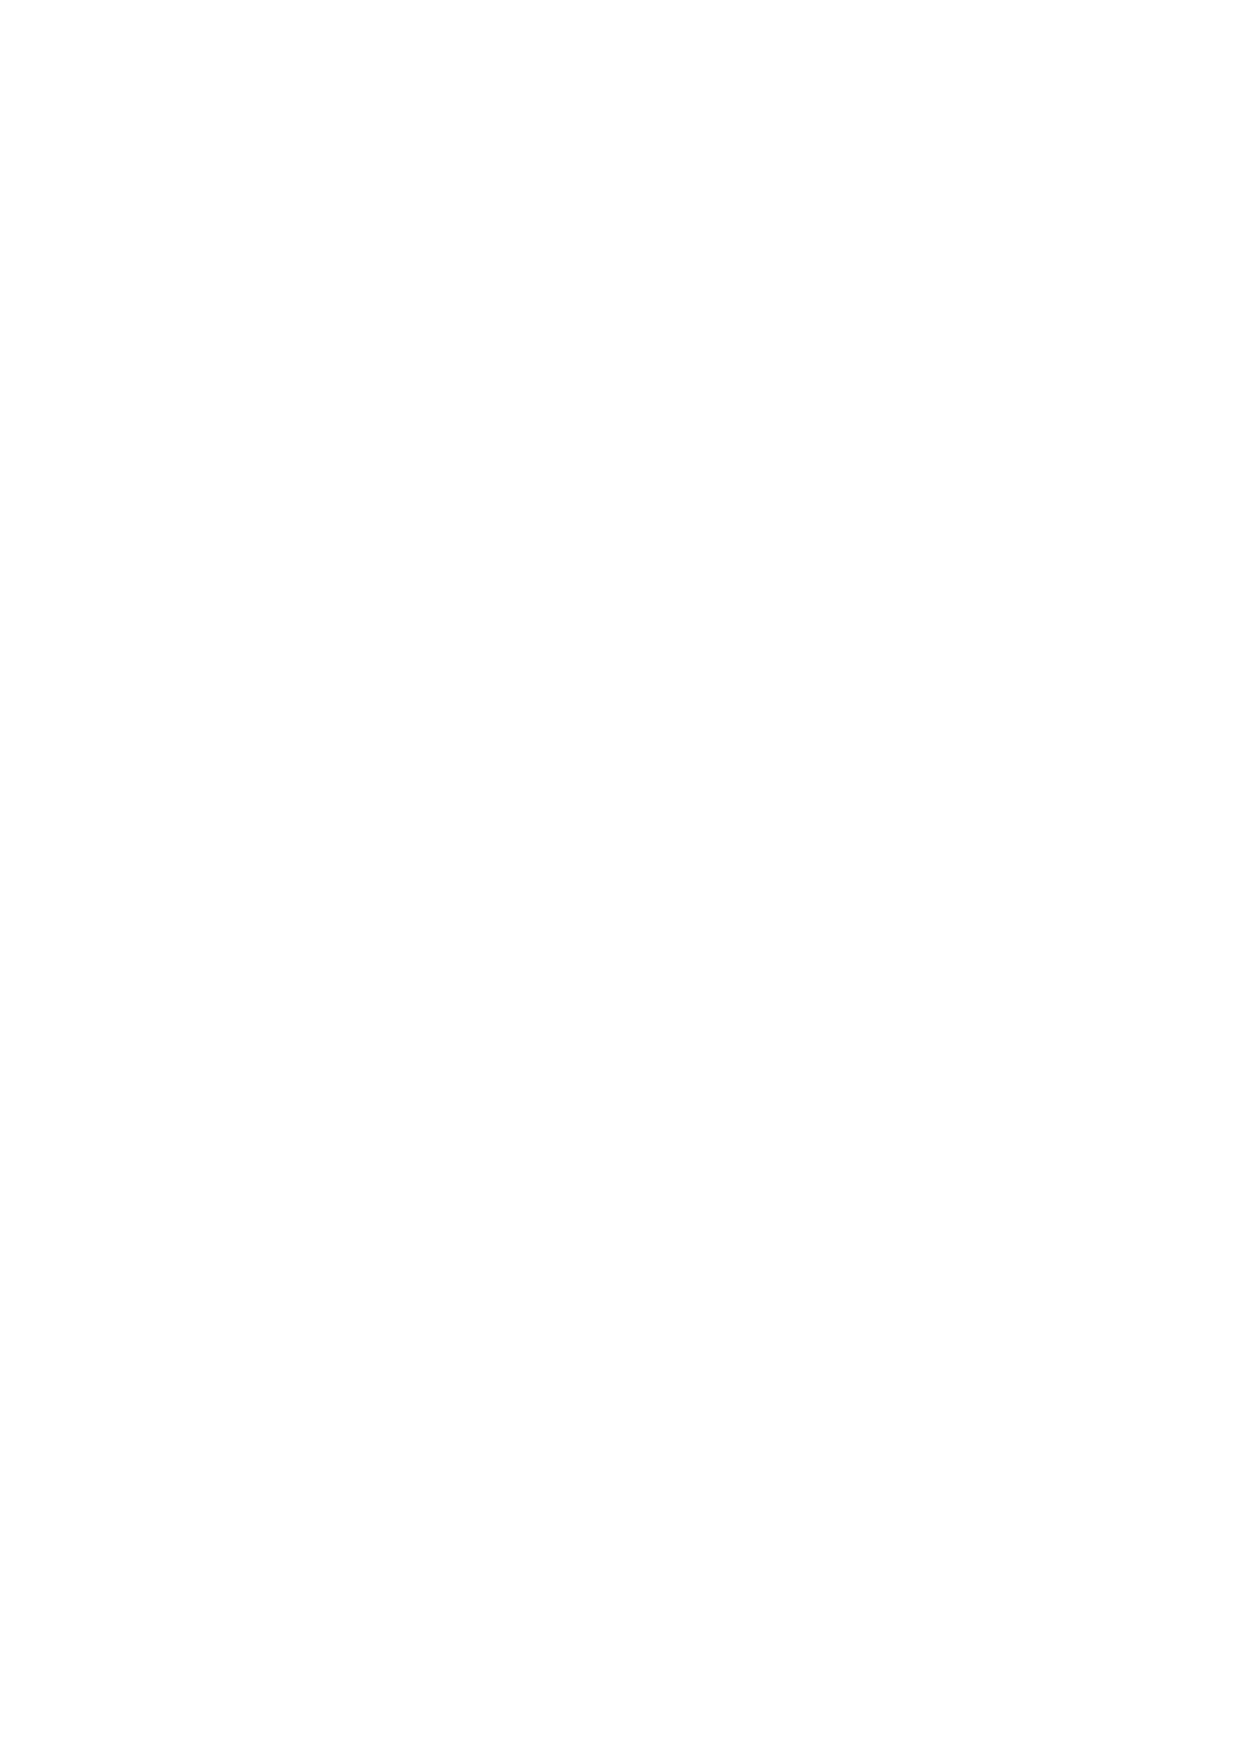
\includegraphics[width=\columnwidth]{./figs/ch2_triang_ar}
		%\vspace*{-10cm}
		\resizebox{\columnwidth}{!}{%Code by GVV Sharma
%December 7, 2019
%released under GNU GPL
%Drawing a triangle given 3 sides

\begin{tikzpicture}
[scale=2,>=stealth,point/.style={draw,circle,fill = black,inner sep=0.5pt},]

%Triangle sides
\def\a{6}
\def\b{5}
\def\c{4}
 
%Coordinates of A
%\def\p{{\a^2+\c^2-\b^2}/{(2*\a)}}
\def\p{2.25}
\def\q{{sqrt(\c^2-\p^2)}}

%Labeling points
\node (A) at (\p,\q)[point,label=above right:$A$] {};
\node (B) at (0, 0)[point,label=below left:$B$] {};
\node (C) at (\a, 0)[point,label=below right:$C$] {};

%Foot of perpendicular

\node (D) at (\p,0)[point,label=above right:$D$] {};

%Drawing triangle ABC
\draw (A) -- node[left] {$\textrm{c}$} (B) -- node[below] {$\textrm{a}$} (C) -- node[above,xshift=2mm] {$\textrm{b}$} (A);

%Drawing altitude AD
\draw (A) -- node[left] {$\textrm{h}$}(D);

%Drawing and marking angles
%\tkzMarkAngle[fill=orange!40,size=0.5cm,mark=](A,C,B)
%\tkzMarkAngle[fill=orange!40,size=0.4cm,mark=](D,B,A)
%\tkzMarkAngle[fill=green!40,size=0.5cm,mark=](B,A,C)
%\tkzMarkAngle[fill=green!40,size=0.5cm,mark=](C,B,D)
\tkzMarkRightAngle[fill=blue!20,size=.2](A,D,B)
%\tkzMarkRightAngle[fill=blue!20,size=.2](B,D,A)
%\tkzLabelAngle[pos=0.65](A,C,B){$\theta$}
%\tkzLabelAngle[pos=0.65](A,B,D){$\theta$}
%\tkzLabelAngle[pos=1](B,A,C){\rotatebox{-45}{$\alpha = 90\degree -\theta$}}
%\tkzLabelAngle[pos=0.65](C,B,D){$\alpha$}

\end{tikzpicture}
}
	\end{center}
	\caption{Area of a Triangle}
	\label{fig:tri_sss}	
\end{figure}

\solution From\eqref{ch2_triang_sum},
\begin{equation}
\label{ch2_triang_ar_1}
ar\brak{ABCD} = ar\brak{ACB} + ar\brak{ADB}
\end{equation}
Also from \eqref{ch2_triang_eq},
\begin{equation}
\label{ch2_triang_ar_2}
ar\brak{ACB} = ar\brak{ADB}
\end{equation}
From \eqref{ch2_triang_ar_1} and \eqref{ch2_triang_ar_2},
\begin{align}
2ar\brak{ACB} &= ar\brak{ABCD} = ac \brak{\text{from} \quad \eqref{fig:tri_rect}}
\\
\Rightarrow ar\brak{ACB} &= \frac{ac}{2}
\end{align}

%
\item In Fig. 	\ref{fig:tri_sss}, $AD \perp BC$.  $AD$ is defined as the {\em altitude}.
\item
	Show that the area of $\Delta ABC$ in Fig. 	\ref{fig:tri_sss}	is $\frac{1}{2}ah$. 


\solution In Fig. \ref{fig:tri_sss},
\begin{align}
ar\brak{\Delta ADC} &= \frac{1}{2}hy \\
ar\brak{\Delta ADB} &= \frac{1}{2}hx 
\end{align}
Thus,
\begin{align}
ar\brak{\Delta ABC} &= ar\brak{\Delta ADC} + ar\brak{\Delta ADB} \\
&= \frac{1}{2}hy + \frac{1}{2}hx = \frac{1}{2}h\brak{x+y} \\
&= \frac{1}{2}ah
\end{align}
%
\item Draw Fig. \ref{fig:tri_sss} with $a=6$, $b=5$  and $c=4$.  
\label{const:tri_sss}
\\
\solution Let the vertices of  $\triangle ABC$ and $\vec{D}$ be 
\begin{align}
\label{eq:tri_basic}
\vec{A} = \myvec{p\\q}, \vec{B} = \myvec{0\\0}, \vec{C} = \myvec{a\\0}, \vec{D} = \myvec{p\\0}
\end{align}
%

Then
\begin{align}
\label{eq:c_tricoord}
AB &= \norm{\vec{A}-\vec{B}}^2 = \norm{\vec{A}}^2  = c^2 \quad \because \vec{B} = \vec{0}
\\
\label{eq:a_tricoord}
BC &= \norm{\vec{C}-\vec{B}}^2 = \norm{\vec{C}}^2  = a^2
\\
AC &= \norm{\vec{A}-\vec{C}}^2 =    b^2
\label{eq:b_tricoord}
\end{align}
%
From \eqref{eq:b_tricoord},
\begin{align}
b^2 &=\norm{\vec{A}-\vec{C}}^2 = \norm{\vec{A}-\vec{C}}^T\norm{\vec{A}-\vec{C}}  
\\
&= \vec{A}^T\vec{A}+\vec{C}^T\vec{C}-\vec{A}^T\vec{C} - \vec{C}^T\vec{A} 
\\
&= \norm{\vec{A}}^2 + \norm{\vec{C}}^2 - 2\vec{A}^T\vec{C} \quad \brak{\because \vec{A}^T\vec{C} = \vec{C}^T\vec{A} } 
\label{eq:tri_const_norm_ac}
\\
&= a^2+c^2-2ap
\end{align}
%
yielding
\begin{align}
p&= \frac{a^2+c^2-b^2}{2a}
\end{align}
%
From \eqref{eq:c_tricoord}, 
\begin{align}
\norm{\vec{A}}^2 &= c^2 = p^2+q^2
\\
\implies q&= \pm \sqrt{c^2-p^2}
\end{align}
%
The python code for  Fig. \ref{fig:tri_sss} is
\begin{lstlisting}
codes/triangle/tri_sss.py
\end{lstlisting}
%
and the equivalent latex-tikz code is
%
\begin{lstlisting}
figs/triangle/tri_sss.tex
\end{lstlisting}
\end{enumerate}
\subsection{Sine and Cosine Formula}
\renewcommand{\theequation}{\theenumi}
\begin{enumerate}[label=\arabic*.,ref=\thesubsection.\theenumi]
\numberwithin{equation}{enumi}

\item
\label{prob:tri_area_sin}
	Show that the area of $\Delta ABC$ in Fig. 	\ref{fig:tri_sss}	is $\frac{1}{2}ab \sin C$.

\solution We have
%
\begin{equation}
ar\brak{\Delta ABC} = \frac{1}{2}ah = \frac{1}{2}ab\sin C \quad \brak{\because \quad h = b \sin C}.
\end{equation}
%
\item
	Show that 
	\begin{equation}
	\frac{\sin A}{a} = \frac{\sin B}{b} = \frac{\sin C}{c}
	\end{equation}

\solution Fig. \ref{fig:tri_sss} can be suitably modified to obtain 
\begin{equation}
ar\brak{\Delta ABC} = \frac{1}{2}ab\sin C = \frac{1}{s}bc\sin A = \frac{1}{2}ca\sin B
\end{equation}
Dividing the above by $abc$, we obtain
	\begin{equation}
\label{eq:tri_sin_form}
	\frac{\sin A}{a} = \frac{\sin B}{b} = \frac{\sin C}{c}
	\end{equation}
This is known as the sine formula.	
%
\item
In Fig. \ref{fig:tri_cosine_formula}, show that
%
\begin{equation}
\label{eq:tri_cos_form}
\cos A = \frac{b^2+c^2-a^2}{2bc}
\end{equation}
%
\

\begin{figure}[!ht]
	\begin{center}
		
		%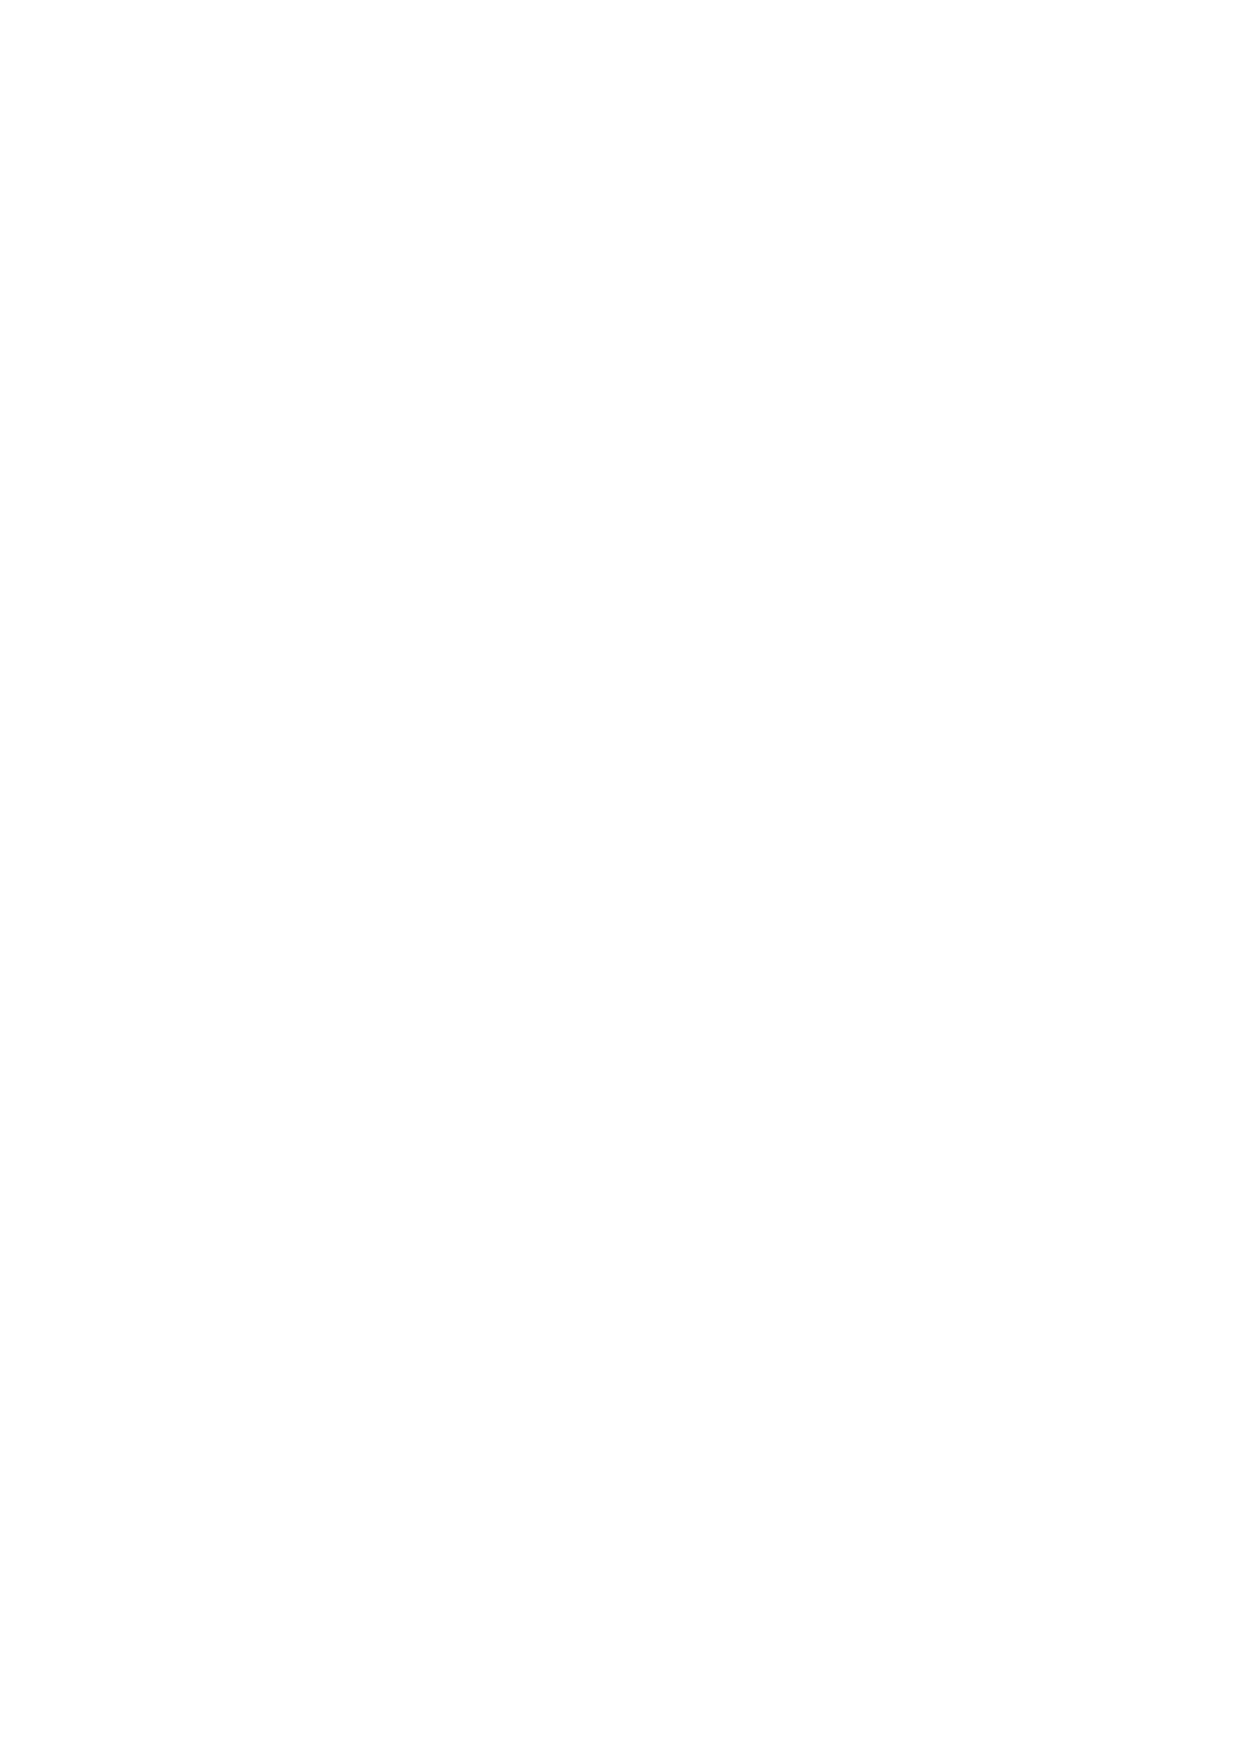
\includegraphics[width=\columnwidth]{./figs/ch2_triang_ar}
		%\vspace*{-10cm}
		\resizebox{\columnwidth}{!}{%Code by GVV Sharma
%December 7, 2019
%released under GNU GPL
%Drawing a triangle given 3 sides

\begin{tikzpicture}
[scale=2,>=stealth,point/.style={draw,circle,fill = black,inner sep=0.5pt},]

%Triangle sides
\def\a{6}
\def\b{5}
\def\c{4}
 
%Coordinates of A
%\def\p{{\a^2+\c^2-\b^2}/{(2*\a)}}
\def\p{2.25}
\def\q{{sqrt(\c^2-\p^2)}}

%Labeling points
\node (A) at (\p,\q)[point,label=above right:$A$] {};
\node (B) at (0, 0)[point,label=below left:$B$] {};
\node (C) at (\a, 0)[point,label=below right:$C$] {};

%Foot of perpendicular

\node (D) at (\p,0)[point,label=above right:$D$] {};

%Drawing triangle ABC
\draw (A) -- node[left] {$\textrm{c}$} (B) -- node[below] {$\textrm{a}$} (C) -- node[above,xshift=2mm] {$\textrm{b}$} (A);

%Drawing altitude AD
\draw (A) -- node[left] {$\textrm{h}$}(D);

\tkzMarkRightAngle[fill=blue!20,size=.2](A,D,B)

\node [below] at ($(B)!0.5!(D)$) {$x$};
\node [below] at ($(C)!0.5!(D)$) {$y$};

\end{tikzpicture}
}
	\end{center}
	\caption{The cosine formula}
	\label{fig:tri_cosine_formula}	
\end{figure}

\solution From Fig. \ref{fig:tri_cosine_formula}, 
%
\begin{align}
a &= x + y = b \cos C + c \cos B.
\end{align}
%
Similarly,
%
\begin{align}
b &= c \cos A + a \cos C \\
c &= b \cos A + a \cos B
\end{align}
%
The above equations can be expressed in matrix form as
%
\begin{equation}
\begin{pmatrix}
0 & c & b \\
c & 0 & a \\
b & a & 0
\end{pmatrix}
\begin{pmatrix}
\cos A \\
\cos B \\
\cos C
\end{pmatrix}
= 
\begin{pmatrix}
a\\
b\\
c
\end{pmatrix}
\end{equation}
%
Using the properties of determinants,
%
\begin{align}
\cos A &= \frac{
\begin{vmatrix}
a & c & b \\
b & 0 & a \\
c & a & 0
\end{vmatrix}
	}
	{
\begin{vmatrix}
0 & c & b \\
c & 0 & a \\
b & a & 0
\end{vmatrix}
	}
	=\frac{ab^2 + ac^2 - a^3}{abc + abc} 
\\
&= \frac{b^2 + c^2 - a^2}{2abc}
\end{align}
%
\end{enumerate}
\subsection{Hero's formula}
\renewcommand{\theequation}{\theenumi}
\begin{enumerate}[label=\arabic*.,ref=\thesubsection.\theenumi]
\numberwithin{equation}{enumi}

\item Find Hero's formula for the area of a triangle.
\\
\solution 
%In Fig. \ref{fig:rt_triangle}, from Baudhayana's theorem, 
%\begin{align}
%\label{eq:tri_geo_baudh}
%b^2 = a^2+c^2 &
%\\
%=b^2\cos^2C+b^2\sin^2C &
%\\
%\implies \cos^2C+\sin^2C &= 1
%\end{align}
%
%In Fig. \ref{fig:tri_const_ex_cos_form}, 
From \eqref{prob:tri_area_sin}, the area of $\triangle ABC$ is 
{\footnotesize
\begin{align}
\label{eq:tri_geo_area_sin_form}
 \frac{1}{2}ab\sin C
%\\
&=\frac{1}{2}ab\sqrt{1-\cos^2C} 
\quad \brak{\text{from } \eqref{eq:tri_sin_cos_id}
%\eqref{eq:tri_geo_baudh}
}
\\
&=\frac{1}{2}ab\sqrt{1-\brak{\frac{a^2+b^2-c^2}{2ab}}^2} \brak{\text{from } \eqref{eq:tri_cos_form}
}
\\
&=\frac{1}{4}\sqrt{\brak{2ab}^2-\brak{a^2+b^2-c^2}}
\\
&=\frac{1}{4}\sqrt{\brak{2ab+a^2+b^2-c^2}\brak{2ab-a^2-b^2+c^2}}
\\
&= \frac{1}{4}\sqrt{\cbrak{\brak{a+b}^2-c^2}\cbrak{c^2-\brak{a-b}^2}}
\\
&= \frac{1}{4}\sqrt{\brak{a+b+c}\brak{a+b-c}\brak{a+c-b}\brak{b+c-a}}
\label{eq:tri_ex_hero_temp}
\end{align}
}
Substituting 
%
\begin{align}
s=\frac{a+b+c}{2}
\end{align}
%
in \eqref{eq:tri_ex_hero_temp}, the area of $\triangle ABC$ is 
%
\begin{align}
\label{eq:tri_area_hero}
\sqrt{s\brak{s-a}\brak{s-b}\brak{s-c}}
\end{align}
%
This is known as Hero's formula.
\item Find the area of $\triangle ABC$ in Fig. \ref{fig:tri_rect}.
\\
\solution The desired are is computed using \eqref{eq:tri_area_hero} by the following 
the python code.
\begin{lstlisting}
codes/triangle/tri_area_hero.py
\end{lstlisting}
%

\item Show that the sum of two sides of a triangle is always greater than the third side.
\\
\solution In \eqref{eq:tri_area_hero}, all terms under the square roots should be positive.  Hence,
%
\begin{align}
\label{eq:tri_hero_ineq}
\begin{split}
s-a &>0
\\
s-b &>0
\\
s-c &>0
\end{split}
\end{align}
resulting in 
%
\begin{align}
\begin{split}
\label{eq:tri_sum_ineq}
b+c &>a
\\
c+a &>b
\\
a+b &>c
\end{split}
\end{align}
\end{enumerate}


